\appsection[Proofs]

The following lemma will allow us to argue that all parties share a common
view of sufficiently old transactions.

\begin{lemma}[Past Perfect]\label{lem:past-perfect}
  Consider a temporal ledger protocol $\Y$'s
  execution $\Exec$ with duration $R$ rounds in which $\Y$ is
  safe, live with liveness $u$, and timely with timeliness $v$.
  If for some honest party $P_1$ and some round $r_1$ it holds that
  $(r^*, \tx) \in \Ledger[P_1][][r_1]$, then
  for all honest parties $P_2$ and for all rounds $r_2 > r^* + v$
  it holds that
  $(r^*, \tx) \in \Ledger[P_2][][r_2]$,
  % TODO:
  % We may be able to remove this extra assumption if
  % we change temporal ledgers to also report their "current time"
  % under the following constraints:
  % 1) In synchronous settings, or after GST in psync, the "current time"
  %    reported by the ledger must not be too far in the past (more than $v$?)
  % 2) The "current time" reported must march only forward;
  %    the next "current time" reported must be larger than the
  %    current "current time" reported.
  % 3) If I read the ledger at some round r_1 and the current time reported
  %    is r_1', then I read the ledger again at round r_2 > r_1, then
  %    any *new* transactions that appear must have a recorded round of
  %    at least r_1'.
  % We may be able to replace "timeliness" completely with the above
  % definition.
  as long as at least one new honest transaction $\tx'$ appears at
  any round $r_1 < r_3 \leq R - u$.
\end{lemma}
\begin{proof}
  Consider an execution as in the statement and suppose, towards a contradiction,
  that $(r^*, \tx) = \Ledger[P_1][][r_1][k]$ for some $k \in \mathbb{N}$,
  but $(r^*, \tx) \not\in \Ledger[P_2][][r_2]$
  with $r^* + v < r_2$.
  From safety,
  $\Ledger[P_2][][r_2] \prec \Ledger[P_1][][r_1]$ and
  $|\Ledger[P_2][][r_2]| \leq k < |\Ledger[P_1][][r_1]|$.
  Due to liveness, $(r', \tx') = \Ledger[P_2][][r_3 + u][k']$,
  for some $r', k' \in \mathbb{N}$.
  As $\tx'$ is new, it is not in $\Ledger[P_1][][r_1]$.
  Due to safety, $k' \geq |\Ledger[P_1][][r_1]| > k$.
  Due to safety, $\Ledger[P_2][][r_3 + u][k] = (r^*, \tx)$.
  Therefore
  $(r^*, \tx) \in \Ledger[P_2][][r_3 + u][|\Ledger[P_2][][r_2]|{:}]$.
  Since $r^* < r_2 - v$, this contradicts the timeliness with parameter $v$.\Qed
\end{proof}

The above property, which follows from safety, liveness, timeliness and
contiguous honest participation is also known in the literature as
\emph{persistence}~\cite{backbone}.

\begin{figure}
  \centering
  \iftwocolumn
  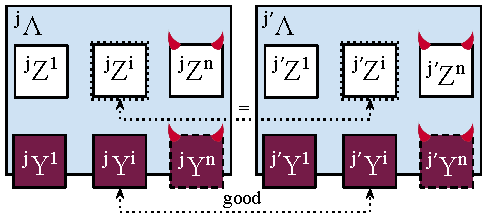
\includegraphics[width=0.7 \columnwidth,keepaspectratio]{figures/rollerblade-cross-party.pdf}
  \else
  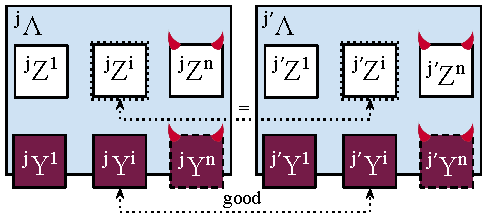
\includegraphics[width=0.6 \columnwidth,keepaspectratio]{figures/rollerblade-cross-party.pdf}
  \fi
  \caption{The Replication Theorem (Theorem~\ref{thm:replication}) states that
  the execution of the emulated machines $\Z[j][i]$ and $\Z[j'][i]$
  across two different compositor parties $\LLambda[j]$ and $\LLambda[j']$
  is consistent, as long as the underlying ledger $\Y[][i]$ is \emph{good}.}
  \label{fig.cross-party}
\end{figure}

\myparagraph[Theorem~\ref{thm:replication}]
\begin{proof}
  The function \emulationSnapshot of party $j$ (resp. party $j'$)
  calls the deterministic function \emulate with overlay party index $i$,
  ledger $\Ledger[j][i][r + v_i]$ (resp. ledger $\Ledger[j'][i][r + v_i]$), emulation round
  $r$, and current round $r + v_i$. The function \emulate runs its main
  \emph{for} loop (Algorithm~\ref{alg.emulate} Line~\ref{alg.emulate:for})
  up to $r$ (inclusive), which consumes data from $\writeboxes[r - 1]$
  and $\inboxes[r - 1]$ and earlier. These are produced by the function
  \prepareEmulationInputs by looking at transactions recorded in $\Ledger[j][i][r + v_i]$
  (resp. $\Ledger[j'][i][r + v_i]$) with recorded round $< r$.
  Because $\Ledger[][i]$ is \emph{good} in $\mathcal{E}$, it is safe, live($u_i$), and timely($v_i$).
  It suffices to show that all transactions with recorded round
  $< r$ are the same in $\Ledger[j][i][r + v_i]$ and $\Ledger[j'][i][r + v_i]$.
  This holds because of Lemma~\ref{lem:past-perfect} invoked with parties $\Y[j][i]$ and $\Y[j'][i]$,
  rounds $r_1 = r_2 = r + v_i$, $r_3 = r + v_i$ and $r^* < r$.
  During round $r_3$, the new honest transaction is due to any honest
  relayer.\Qed
\end{proof}

\myparagraph[Lemma~\ref{lem:consistency}]
\begin{proof}
  Let $i \in H$, $r \geq 0$, $r + \Delta_v < r' < R$ be arbitrary.
  When $\emulationSnapshot$ is invoked at the end of round $r'$ (resp. $r' + 1$),
  the value $\this.\now$
  is $r'$ (resp. $r' + 1$), so the check $\emulationRound > \this.\now - v_i$ of Algorithm~\ref{alg.prepare-emulation-inputs}
  Line~\ref{alg.prepare-emulation-inputs:reality-lag} is \emph{false}, and the emulation
  succeeds. This is the only stateful check in this function.
  The result of the function $\prepareEmulationInputs$ only depends on the transactions of
  its $\Ledger[j][i]$ argument with recorded rounds up to $\emulationRound$.
  Therefore it suffices to show that the transactions in
  $\Ledger[j][i][r']$ with recorded rounds up to $\emulationRound$ are the same
  as the transactions in $\Ledger[j][i][r' + 1]$ with recorded rounds up to $\emulationRound$.
  All $\Ledger[j][i][r']$ transactions with recorded rounds up to $\emulationRound$
  are included in $\Ledger[j][i][r' + 1]$ by \emph{stickiness}.
  Conversely, all $\Ledger[j][i][r' + 1]$ transactions with recorded rounds up to $\emulationRound$
  are included in $\Ledger[j][i][r']$ by \emph{timeliness}.\Qed
\end{proof}

\myparagraph[Conjecture~\ref{conj:emulation}]
\begin{proof}[Sketch]
  Let $\Pi$, $\mathcal{Y}$, $\mathcal{B}$ and $\mathcal{H}$
  be as in the statement, and $\Delta =  2 \Delta_v + \Delta_u$.
  Let the adversary $\mathcal{A}$, the belief $B \in \mathcal{B}$,
  and the environment $\mathcal{Z}$, the number of compositor parties $m$,
  and the index of the compositor $j$ of interest be arbitrary
  as in the statement, and set $H = \mathcal{H}(B)$.
  Let $\mathcal{E}$ and $\mathcal{E}'$ be the emulated and party setting
  executions, respectively, sampled as in Definition~\ref{def:faithfulness}.
  As $\Pi$ is a \rollerblade-suitable-overlay protocol it is deterministic.

  We will prove faithfulness by
  construction of the simulator $\mathcal{S}$ and environment $\mathcal{Z}'$.

  % TODO: consider removing the environment $\mathcal{Z}'$
  The simulator $\mathcal{S}$ and environment $\mathcal{Z}'$ work in tandem
  as follows.
  Initially, $\mathcal{S}$ samples an execution
  $\mathcal{E}^*$ in the emulation setting from
  % TODO: is the number of validators in \Y[][1] hard-coded into it?
  $\LCExec_m(\Lambda,\allowbreak\mathcal{Y},\allowbreak\mathcal{A},\allowbreak\mathcal{Z})$
  (see Figure~\ref{fig.conj.simulation}).
  Let $R$ be the duration of $\mathcal{E}^*$ in rounds.
  The simulator looks at compositor party $j$ of $\mathcal{E}^*$
  and its $\Y[j][1], \ldots, \Y[j][n]$.
  The environment $\mathcal{Z}'$ chooses the duration, in rounds, of
  $\mathcal{E}'$ to be $R - \Delta_v - 1$. It initializes $n$
  parties $\PPi[1], \ldots, \PPi[i], \ldots, \PPi[n]$ by invoking
  the \emph{constructor} method with parameters $\Delta, i, n$.

  \begin{figure}
    \centering
    \iftwocolumn
    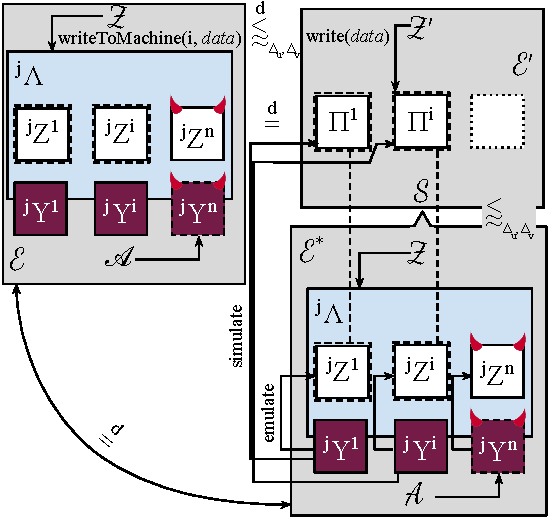
\includegraphics[width=0.9 \columnwidth,keepaspectratio]{figures/rollerblade-emulation.pdf}
    \else
    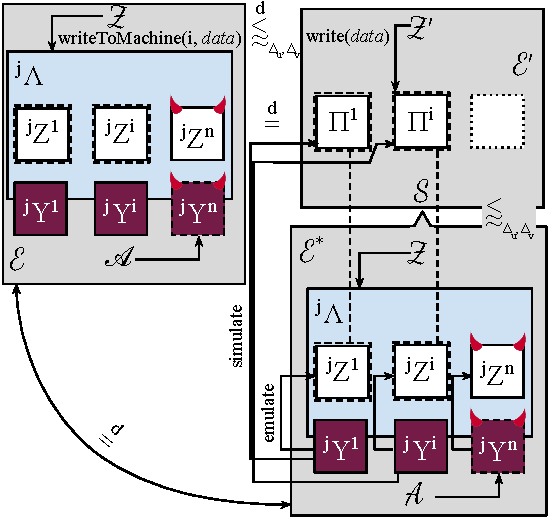
\includegraphics[width=0.7 \columnwidth,keepaspectratio]{figures/rollerblade-emulation.pdf}
    \fi
    \caption{A visualization of the argument that \rollerblade is faithful.
    In the proof of Conjecture~\ref{conj:emulation},
    the simulator $\mathcal{S}$ and simulated environment $\mathcal{Z}'$
    give rise to execution $\mathcal{E}'$ in the
    party setting (top right) by sampling an execution $\mathcal{E}^*$ in the emulated
    setting with adversary $\mathcal{A}$ and environment $\mathcal{Z}$
    (bottom right). The simulator uses each good ledger $\Y[i][j]$ in
    $\mathcal{E}^*$ to feed data into the respective honest party $\PPi[i]$
    in $\mathcal{E}'$. }
    \label{fig.conj.simulation}
  \end{figure}

  % TODO: consider moving the simulation to an algorithm/figure
  The simulator initially obtains, for every $i \in [n]$,
  a copy of the configuration $M_i$ of the ITI $\RB[j]$ from $\mathcal{E}^*$ at the end of
  $\mathcal{E}^*$.
  The simulator calls $\prepareEmulationInputs(i, \emulationRound, \realityRound)$ on $M_i$
  \emph{in vitro} at the end of round $R$, where $\emulationRound = R - \Delta_v - 1$
  and $\realityRound = R$, to obtain the pair
  $(\writeboxes^i, \inboxes^i)$, where
  $|\writeboxes^i| = R - \Delta_v - 1$
  and
  $|\inboxes^i| = R - \Delta_v - 1$.
  At the beginning of round $r$ of $\mathcal{E}'$, the simulator calls
  $\lwrite(\data)$ on party $i$
  for every $\data \in \writeboxes^i[r - 1]$.
  At every round, $\mathcal{Z}'$ activates each party, in order,
  by invoking $\PPi[i].\execute()$.
  If party $\PPi[i]$ invokes the network receive method $\recv()$, while active,
  then $\mathcal{Z}'$ provides $\inboxes^i[r - 1]$.
  If $\PPi[i]$ invokes the network send method $\send(i', \msg)$, while active,
  then it is ignored by $\mathcal{Z}'$.

  % TODO: separate the notion of "emulation" and the notion of "simulation"

  We note that $\mathcal{S}$ uses the adversary $\mathcal{A}$ and the
  environment $\mathcal{Z}$ in this simulation, so $\mathcal{E}$
  and $\mathcal{E}^*$ are identically distributed.
  For (1) it suffices to show that for all $j$,
  $\LCView_{j,H,\Delta_v}(\mathcal{E}^*) = \PEView_H(\mathcal{E}')$
  (i.e., we will show the these two random variables are equal,
  not just equal by distribution),
  and similarly for (2) it suffices to show that for all $j$,
  $\LCExtern_j(\mathcal{E}^*) \laterly{\Delta_u,\Delta_v} \PEExtern(\mathcal{E}')$
  (i.e., we will show that the externalities of $\mathcal{E}'$ are
  similar to $\mathcal{E}^*$, not just \emph{distributionally} similar).
  See Figure~\ref{fig.emulation-distribution}.

  \begin{figure}
    \centering
    \iftwocolumn
    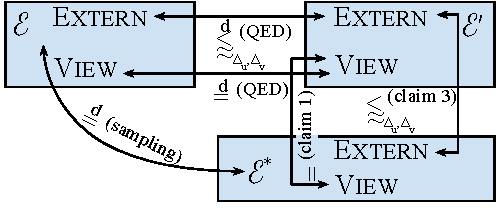
\includegraphics[width=0.8 \columnwidth,keepaspectratio]{figures/rollerblade-emulation-distribution.pdf}
    \else
    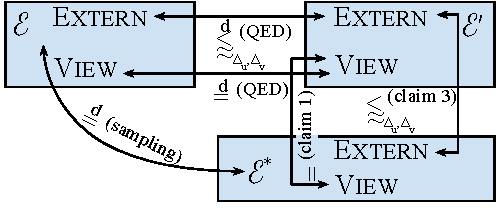
\includegraphics[width=0.6 \columnwidth,keepaspectratio]{figures/rollerblade-emulation-distribution.pdf}
    \fi
    \caption{The environments $\mathcal{Z}$ in $\mathcal{E}$ and $\mathcal{Z}'$
    in $\mathcal{E}'$ respectively
    give rise to externalities similar in distribution ($\laterlydistr{\Delta_u,\Delta_v}$,
    middle top),
    whereas the views of the honest parties in $\mathcal{E}$
    and $\mathcal{E}'$ are distributionally equivalent ($\distreq$, middle top).
    The executions $\mathcal{E}$ and $\mathcal{E}^*$ are sampled
    from the same distribution ($\distreq$, bottom left).
    The views of the honest parties in $\mathcal{E}^*$ and $\mathcal{E}'$
    are equal (not just equal in distribution)
    and the externalities in $\mathcal{E}^*$ and $\mathcal{E}'$
    similar (not just similar in distribution).}
    \label{fig.emulation-distribution}
  \end{figure}

  Since $\mathcal{Z}$ is $B$-respecting, therefore $B(\mathcal{E}^*)$ holds.
  Hence, for all $i \in H$, $\Y[][i]$ is safe, live $(u_i)$, and timely $(v_i)$
  in $\mathcal{E}^*$.

  \myparagraph[Claim 1: $\LCView_{j,H,\Delta_v}(\mathcal{E}^*) = \PEView_H(\mathcal{E}')$]
  Let $V^* = \LCView_{j,H,\Delta_v}(\mathcal{E}^*)$ and
  $V' = \PEView_H(\mathcal{E}')$.
  We know that $\mathcal{E}^*$ is $(j, H, \Delta_v)$-consistent
  from Lemma~\ref{lem:consistency}, and so $V^*$
  is well-defined.
  The two views have the same size.
  We need to show
  that the views of all \emph{honest} parties in the two executions are identical.
  Let $i$ be an arbitrary party in $H$.

  Let $c^*(r_1, r_2, r_3)$ denote the configuration
  of the machine $\Z[j][i]$ after the invocation of
  Algorithm~\ref{alg.emulate} Line~\ref{alg.emulate:execute}
  during the $r_3$-rd iteration of the \emph{for loop} in
  Algorithm~\ref{alg.emulate} Line~\ref{alg.emulate:for}
  (or, if $r_3 = 0$, we set $c^*(r_1, r_2, r_3)$ to be the state of
  $\Z[j][i]$ before the \emph{for loop})
  when $\emulationSnapshot$ is
  invoked \emph{in vitro} after round $r_1$ of execution $\mathcal{E}^*$,
  where $r_2 + \Delta_v \leq r_1 \leq R + \Delta_v$ with parameter
  $\emulationRound = r_2$, and $r_3 \leq r_2$.
  This causes an invocation of \emulate with parameters
  $\emulationRound = r_2$ and $\realityRound = r_1$.
  Let $c'(r_3)$ denote the configuration of the machine $\PPi[i]$
  in $\mathcal{E}'$ at the end of round $r_3$.
  We set $c'(0)$ to be the initial configuration of $\PPi[i]$,
  after it's \emph{constructor} is invoked.

  We will prove that $V^*_{i,r} = V'_{i,r}$ by induction on $r$.
  Let $r$ be an arbitrary round such that $1 \leq r \leq R - \Delta_v - 1$.

  If $r = 1$, then
  \begin{equation}\label{conj:emulation:ind-hyp}
    c^*(r + \Delta_v, r - 1, r - 1) = c'(r - 1)\,
  \end{equation}
  because the state of machine $\Z[j][i]$ and $\PPi[i]$ are identical
  after the initial invocation of the \emph{constructor} as $\Pi$
  is deterministic.

  If $r > 1$, then by inductive hypothesis we have $V^*_{i,r - 1} = V'_{i,r - 1}$
  by which Eq~\ref{conj:emulation:ind-hyp} also follows.

  In either case, Eq~\ref{conj:emulation:ind-hyp} holds, and we
  wish to show that $c^*(r + \Delta_v, r, r) = c'(r)$,
  from which it will follow that $V^*_{i,r} = V'_{i,r}$.

  \begin{figure*}
    \centering
    \iftwocolumn
    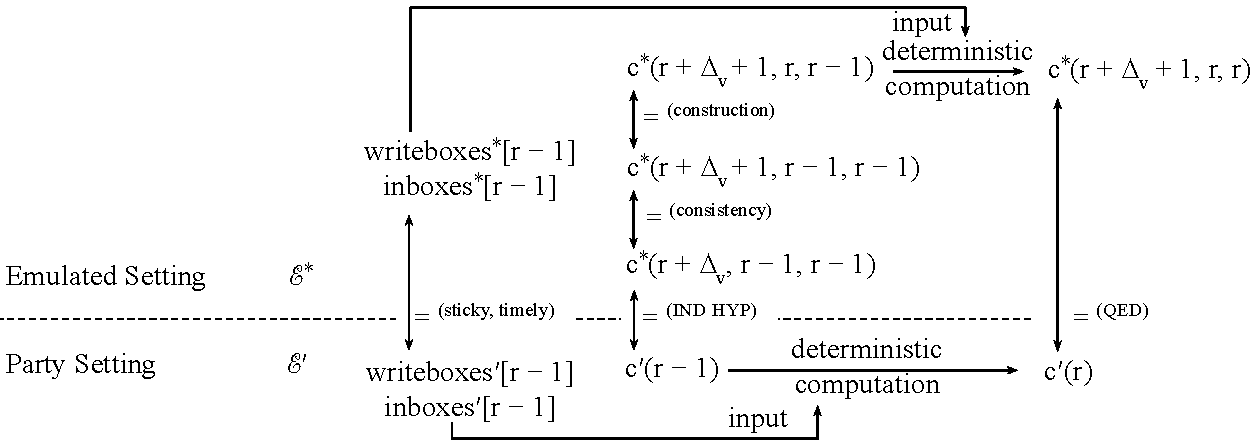
\includegraphics[width=0.6 \textwidth,keepaspectratio]{figures/emulation-claim-1-induction.pdf}
    \else
    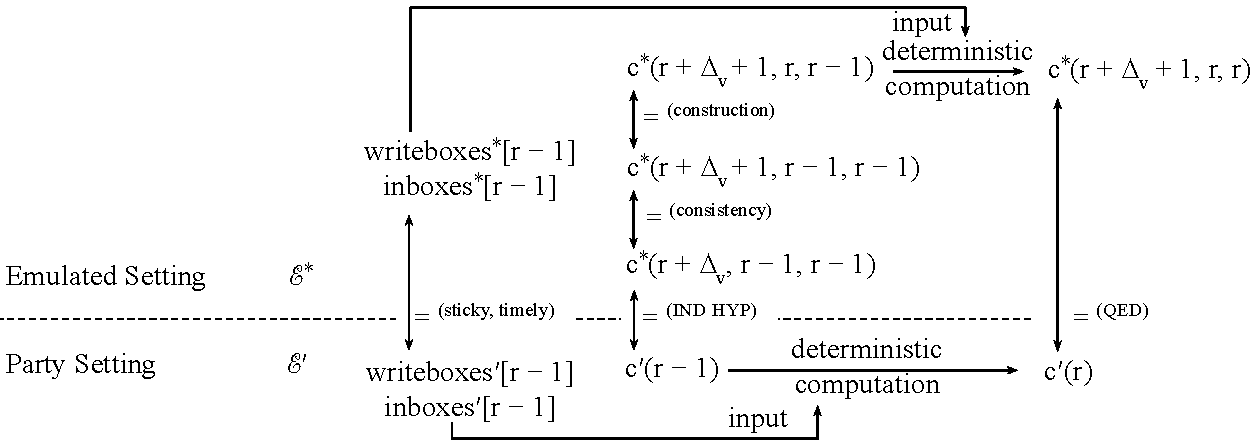
\includegraphics[width=\textwidth,keepaspectratio]{figures/emulation-claim-1-induction.pdf}
    \fi
    \caption{The inductive step in the proof of the Emulation Conjecture.}
    \label{fig.emulation-claim-1-induction}
  \end{figure*}

  Because $\mathcal{E}^*$ is consistent, we have that
  \begin{equation}\label{conj:emulation:consistency}
    c^*(r + \Delta_v, r - 1, r - 1) = c^*(r + \Delta_v, r - 1, r - 1)\,.
  \end{equation}
  Each iteration of the \emph{for} loop of Algorithm~\ref{alg.emulate} Line~\ref{alg.emulate:for}
  proceeds until the round reaches $\emulationRound$, therefore
  $c^*(r + \Delta_v, r, r - 1) = c^*(r + \Delta_v, r - 1, r - 1)$.
  From this and Eq~\ref{conj:emulation:consistency} we conclude that
  $c^*(r + \Delta_v, r, r - 1) = c^*(r + \Delta_v, r - 1, r - 1)$.
  From this and Eq~\ref{conj:emulation:ind-hyp} we conclude that
  \begin{equation}\label{conj:emulation:pre-state}
    c^*(r + \Delta_v, r, r - 1) = c'(r - 1)\,.
  \end{equation}

  Let $(\writeboxes^*, \inboxes^*)$
  be the pair
  returned by the invocation of $\prepareEmulationInputs(i, \Ledger[j][i][r + \Delta_v], r)$
  \emph{in vitro} after round $r + \Delta_v$ for party $\LLambda[j]$ of $\mathcal{E}^*$, and, likewise define
  $(\writeboxes', \inboxes')$ to be the pair
  returned by the invocation of $\prepareEmulationInputs(i, \Ledger[j][i][R], R - \Delta_v - 1)$
  \emph{in vitro} after round $R$ of $\mathcal{E}^*$ on party $\LLambda[j]$.
  Because $\Y[j][i]$ in $\mathcal{E}^*$ is \emph{sticky} and \emph{timely}$(v_i)$
  the transactions in
  $\Ledger[j][i][r + \Delta_v]$ with recorded round $r - 1$ are identical to
  the transactions in $\Ledger[j][i][R]$ with recorded round $r - 1$
  (all transactions with recorded round $r - 1$ of $\Ledger[j][i][r + \Delta_v]$
   will appear in $\Ledger[j][i][R]$ by stickiness;
   and all transactions with recorded round $r - 1$ of $\Ledger[j][i][R]$ will
   have appeared in $\Ledger[j][i][r + \Delta_v]$ by timeliness; in the case of
   $r = 1$, no transactions with recorded round $r - 1$ will appear in either
   ledger).
  Hence,
  \begin{align}
    \writeboxes^*[r - 1] &= \writeboxes'[r - 1]\label{conj:emulation:eq-inputs-writes}\\
    \inboxes^*[r - 1] &= \inboxes'[r - 1]\label{conj:emulation:eq-inputs-inboxes}\,,
  \end{align}
  since the loop of Algorithm~\ref{alg.prepare-emulation-inputs} Line~\ref{alg.prepare-emulation-inputs:for}
  will run identically in the two invocations of $\prepareEmulationInputs$ up to
  and including round $r - 1$ (and for
  $r = 1$, $\writeboxes^*[0] = \inboxes^*[0] = \writeboxes'[0] = \inboxes'[0]$ by construction).

  By the \rollerblade construction,
  $c^*(r + \Delta_v, r, r)$ is the result of
  taking the machine configuration
  $c^*(r + \Delta_v, r, r - 1)$
  and running the \emph{for} loop of Algorithm~\ref{alg.emulate} Line~\ref{alg.emulate:for}
  for one more iteration, providing inputs $\writeboxes^*[r - 1], \inboxes^*[r - 1]$
  during the execution of $\Z[j][i]$.
  To see why $\writeboxes^*, \inboxes^*$ in particular are used in this iteration,
  note that these correspond to the invocation of $\prepareEmulationInputs$ in
  Algorithm~\ref{alg.emulate} Line~\ref{alg.emulate:recursion}.

  Similarly, by the simulator construction, % TODO: when does the simulator obtain \writeboxes, \inboxes? In vitro R...
  the simulator evolves the machine $\PPi[i]$ in $\mathcal{E}'$ from round $r - 1$,
  in which it has configuration $c'(r - 1)$,
  to round $r$,
  in which it has configuration $c'(r)$,
  by feeding it the inputs $\writeboxes'[r - 1], \inboxes'[r - 1]$.

  As $c^*(r + \Delta_v, r, r - 1) = c'(r - 1)$ (by Eq~\ref{conj:emulation:pre-state})
  and the two configurations evolve using the same inputs (by
  Eqs~\ref{conj:emulation:eq-inputs-writes} and \ref{conj:emulation:eq-inputs-inboxes}),
  and, since $\Pi$ is deterministic,
  therefore $c^*(r + \Delta_v, r, r) = c'(r)$ (see Figure~\ref{fig.emulation-claim-1-induction}).
  We conclude that $V^*_{i,r} = V'_{i,r}$, completing the induction
  and the proof of Claim 1.

  \myparagraph[Claim 2: $\mathcal{Z}'$ respects the network model]
  Namely, the claim is that for all $i, i' \in H$, for all rounds $r$ of $\mathcal{E}'$:

  \begin{enumerate}[label=(\alph*)]
    \item
    \label{conj:emulation:claim-delta-a}
    If $\PPi[i]$ sends a message to $\PPi[i']$ at round $r$, then this message is delivered to $\PPi[i']$
    (with source $i$) between round $r + 1$ and $r + \Delta$, and

    \item
    \label{conj:emulation:claim-delta-b}
    If $\PPi[i']$ received a message from $\PPi[i]$ at round $r^*$, then this message was sent by $\PPi[i]$.
  \end{enumerate}

  We will first prove that for all $i, i' \in H$, for all rounds $r$

  Let round $r^* > r + v_i + u_{i'}$.

  When $\LLambda[j].\prepareEmulationInputs(i', \Ledger[j][i'][R], R)$ is called in vitro
  at the end of round $R + \Delta_v$, after Line~\ref{alg.prepare-emulation-inputs:set-f} of Algorithm~\ref{alg.prepare-emulation-inputs},
  it holds that all transactions with recorded round up to $r - v_i - u_{i'} - 1$ that are included in $F^{i}$ are also included in $\Ledger[j][i][r + v_i]$.


  Let $r$ be the round during which $\PPi[i]$ sends message $\msg$ to $\PPi[i']$.
  That means that $\PPi[i]$ invoked network function $\send(i', \msg)$ at round $r$.
  In Claim 1, we showed that the transcript of machine $\PPi[i]$ in $\mathcal{E}'$
  is identical to the transcript of machine $\Z[j][i] = \LLambda[j].\emulationSnapshot(i,r)$ in $\mathcal{E}^*$
  called in vitro at the end of round $r + \Delta_v$.
  Hence, $\Z[j][i]$ also invoked network function $\send(i', \msg)$ at round $r$.
  This means that $\{\textsf{to}: i', \msg: \msg\} \in \LLambda[j].\emulate(i, \Ledger[j][i][r + \Delta_v], r).\outboxes[r]$.

  % At the beginning of round $r$, environment $\mathcal{Z}'$
  % calls $\lwrite(\data)$ on party $i$.

  % Then, $\PPi[i]$ is activated
  % is provided

  % At round $r$, $\PPi[i]$ is activated by $\mathcal{Z}'$ and
  % has $\inboxes^i[r - 1]$

  %TODO: Add encode/decode?
  At round $r + v_i$, relayer $\LLambda[j]$ invokes $\relay()$.
  This creates a transcription $\tau = \Y[j][i].\transcribe()$, where
  $\Y[j][i].\untranscribe(\tau) = \Ledger[j][i][r + v_i]$.
  Then, it transmits a new bulletin `chkpt'
  transaction $\tx$, encoding instruction $\instruction$ containing transcription $\tau$ to $\Y[][i']$.

  Because of the liveness of $\Y[][i']$,
  transaction $\tx$ appears in $\Ledger[j][i']$, for the first time,
  at round $r' \leq r + v_i + u_{i'}$.
  Hence, $(\hat{r}, \tx) \in \Ledger[j][i'][r']$, where $\hat{r}$ is the recorded round of $\tx$
  and $\hat{r} \leq r'$. Because of the stickiness of $\Y[][i']$, transaction $(\hat{r}, \tx)$ will
  appear in $\Ledger[j][i'][R]$ in the same position as in $\Ledger[j][i'][r']$.

  Party $\LLambda[j]$ will relay $\Y[][i]$ at round $r + v_i + v_{i'}$, and
  because of the liveness of $\Y[][i']$, it will appear on $\Ledger[j][i']$ for the
  first time no later than round $r + v_i + u_{i'} + v_{i'}$ with recorded round
  after $r + v_i + u_{i'}$ but no later than $r + v_i + u_{i'} + v_{i'}$.

  Let $(r^*, \tx^*)$ be the first bulletin `chkpt' transaction from $\Y[][i]$ in $\Ledger[j][i'][R]$, such that
  $r^* > r + v_{i} + u_{i'} \geq r' \geq \hat{r}$. It holds that $r^* \leq r + v_{i} + u_{i'} + v_{i'}$.

  The simulator calls \emph{in vitro} (at the end of round $R$)
  $\LLambda[j].\prepareEmulationInputs(i', \Ledger[j][i'][R], R - \Delta_v - 1)$.

  The \emph{for} loop in Algorithm~\ref{alg.prepare-emulation-inputs}
  Line~\ref{alg.prepare-emulation-inputs:for} is eventually entered with
  parameters $(\hat{r}, \instruction)$.
  In Line~\ref{alg.prepare-emulation-inputs:untranscribe}, transcription $\tau$
  is untranscribed and we get $\ImaginaryLedger[j][i'] = \Ledger[j][i][r + v_i]$.
  This means that after Line~\ref{alg.prepare-emulation-inputs:set-f} is executed,
  it holds that $\Ledger[j][i][r + v_i] \preceq F^i$ by the safety of $\Y[][i]$.

  Because, $\hat{r} < r^*$, the \emph{for} loop in Algorithm~\ref{alg.prepare-emulation-inputs}
  is later entered with parameters $(r^*, \tx^*)$.
  After Line~\ref{alg.prepare-emulation-inputs:set-f} is executed,
  it still holds that $\Ledger[j][i][r + v_i] \preceq F^i$.
  Hence, in Line~\ref{alg.prepare-emulation-inputs:recursion}, where
  $\LLambda[j].\emulate(i, F^i, r^* - v_i - u_{i'} - 1)$ is invoked, it holds that
  $\{\textsf{to}: i', \msg: \msg\} \in \LLambda[j].\emulate(i, F^i, r^* - v_i - u_{i'} - 1).\outboxes[r]$
  because $r^* - v_i - u_{i'} - 1 \geq r$.
  By the minimality of $(r^*, \tx^*)$, the $\msg$ will be included in $\inboxes[r^*]$.
  The environment $\mathcal{Z}'$ will provide $\msg$ to $\PPi[i']$
  if network method $\recv()$ is invoked at round $r^*$.

  We conclude that since $\msg$ sent at $r$ was delivered at $r^*$,
  and $r^* \leq r + v_{i} + u_{i'} + v_{i'} \leq r + 2 \Delta_v + \Delta_u \leq r + \Delta$, the
  delay is respected. We observe that the delay for every message is always
  greater than $u_i + v_{i'}$.

  This completes the proof of \ref{conj:emulation:claim-delta-a}.

  Let $\msg$ be the message that $\PPi[i']$ received from $\PPi[i]$ at round $r^*$.
  To prove \ref{conj:emulation:claim-delta-b}, it suffices to show that
  $\PPi[i]$ invoked network function $\send(i', \msg)$ at some round $r$.

  In order for $\PPi[i']$ to receive $\msg$ at round $r^*$,
  the environment $\mathcal{Z}'$ must provide it if network method $\recv()$ is invoked.
  Hence, the $\msg$ must be included in $\inboxes[r^*]$ after $\LLambda[j].\prepareEmulationInputs(i', \Ledger[j][i'][R], R - \Delta_v - 1)$
  is called \emph{in vitro} at the end of round $R$ by the simulator.
  Therefore, there is a bulletin `chkpt' transaction $(r^*, \tx^*)$, such that
  when the \emph{for} loop in Algorithm~\ref{alg.prepare-emulation-inputs} Line~\ref{alg.prepare-emulation-inputs:for}
  is entered with it as parameter, it holds that
  $\{\textsf{to}: i', \msg: \msg\} \in \LLambda[j].\emulate(i, F^{i'}, r^* - v_i - u_{i'} - 1).\outboxes[r]$,
  where $r \leq r^* - v_i - u_{i'} - 1$.

  At round $r^* - u_{i'} - 1$, relayer $\LLambda[j]$ invokes $\relay()$.
  This creates a transcription $\tau = \Y[j][i].\transcribe()$, where
  $\Y[j][i].\untranscribe(\tau) = \Ledger[j][i][r^* - u_{i'} - 1]$.
  Then, it transmits a new bulletin `chkpt' transaction $\tx$,
  encoding instruction $\instruction$ containing transcription $\tau$ to $\Y[][i']$.

  Because of the liveness of $\Y[][i']$, transaction $\tx$ appears on $\Ledger[j][i']$ for the
  first time no later than round $r^* - 1$ and with recorded round $\hat{r} < r^*$, due to timeliness.
  Hence, the \emph{for} loop in Algorithm~\ref{alg.prepare-emulation-inputs}
  Line~\ref{alg.prepare-emulation-inputs:for} is eventually entered with
  parameters $(\hat{r}, \instruction)$.
  In Line~\ref{alg.prepare-emulation-inputs:untranscribe}, transcription $\tau$
  is untranscribed and we get $\ImaginaryLedger[j][i'] = \Ledger[j][i][r^* - u_{i'} - 1]$.
  This means that after Line~\ref{alg.prepare-emulation-inputs:set-f} is executed,
  it holds that $\Ledger[j][i][r^* - u_{i'} - 1] \preceq F^{i'}$ by the safety of $\Y[][i]$.
  Because $r + v_i \leq r^* - u_{i'} - 1$, it holds that $\Ledger[j][i][r + v_i] \preceq F^{i'}$

  Since round $\hat{r}$ precedes round $r^*$, when the \emph{for} loop in Algorithm~\ref{alg.prepare-emulation-inputs}
  is later entered with parameters $(r^*, \tx^*)$, and after Line~\ref{alg.prepare-emulation-inputs:set-f} is executed,
  it still holds that $\Ledger[j][i][r + v_i] \preceq F^{i'}$.
  % All transactions with recorded round up to $r$ are included in $\Ledger[j][i][r + v_i]$ due to timeliness.
  %
  Hence, it holds that
  $\LLambda[j].\emulate(i, F^{i'}, r^* - v_i - u_{i'} - 1).\outboxes[r] = \LLambda[j].\emulate(i, \Ledger[j][i][r + v_i], r).\outboxes[r]$.
  That means that $\Z[j][i]$ invoked network function $\send(i', \msg)$ at round $r$.
  In Claim 1, we showed that the transcript of machine $\PPi[i]$ in $\mathcal{E}'$
  is identical to the transcript of machine $\Z[j][i] = \LLambda[j].\emulationSnapshot(i,r)$ in $\mathcal{E}^*$
  called in vitro at the end of round $r + \Delta_v$.
  Hence, $\PPi[i]$ also invoked network function $\send(i', \msg)$ at round $r$.

  % TODO: double check the exact numbers in this proof
  \myparagraph[Claim 3: $\LCExtern_{j,H}(\mathcal{E}^*) \laterly{\Delta_u,\Delta_v} \PEExtern(\PEView_{\mathcal{H}(B)}(\mathcal{E}'))$]

  Let $i \in H$ and $r \leq R - \Delta_u - \Delta_v - 1$ be arbitrary, and $W^i_r$ be the writebox
  at position $(i, r)$ of $\LCExtern(\mathcal{E}^*)$. Let $m$ be an arbitrary message
  in $W^i_r$. Message $m$ was included in a \emph{writeToMachine} call to $\RB[j]$
  with parameter $i$ at round $r$. By the rollerblade construction, the \emph{write}
  function of $\Y[j][i]$ will be called by $\RB[j]$ at round $r$ with parameter a bulletin
  transaction $\tx$ with payload $(\text{`write'}, m)$. Because bulletin transactions are high entropy,
  this transaction is fresh, namely it does not appear in $\Ledger[j][i][r]$.
  Because $i$ is \emph{good}, therefore it is live in $\mathcal{E}^*$ with liveness $u_i$,
  therefore $\tx$ will appear in $\Ledger[j][i][r + u_i]$ with some recorded round $r^*$.
  Note that round $r + u_i \leq R$ falls within the duration of $\mathcal{E}^*$, and
  so the ledger $\Ledger[j][i][r + u_i]$ can be obtained by the simulator.
  Because $i$ is \emph{timely} in $\mathcal{E}^*$ with timeliness $v_i$, therefore
  $r + 1 - \Delta_v \leq r + 1 - v_i \leq r^* \leq r + u_i \leq r + \Delta_u \leq R - \Delta_v - 1$.
  When the function $\prepareEmulationInputs$ is invoked at $\realityRound = R$
  and with $\emulationRound = R - \Delta_v - 1$, the transaction will contribute
  to the \emph{writebox} of party $i$, since $r^* \leq R - \Delta_v - 1$.
  Hence, $m$ will be inputted to the \emph{write} function call of $\Pi^i$
  in $\mathcal{E}'$ at round $r^*$ (and note that $1 \leq r^* \leq R - \Delta_v - 1$ falls
  within the duration of $\mathcal{E}'$), completing the proof of Claim 3.
  \Qed
  % TODO: Check that there are sufficient rounds before the end of the simulation
  % for $\Pi^i$ to write this message (i.e., for the message to appear in the prepareEmulationInputs
  % output).
\end{proof}
